\section{Data}
    
    \frame{\sectionpage}
    
    \begin{frame}{\textit{Treatment:} The Anti-corruption Program in Brazil}
    
    \begin{columns}

    \begin{column}{0.5\textwidth}
        \begin{figure}\label{fig1}
        \centering
        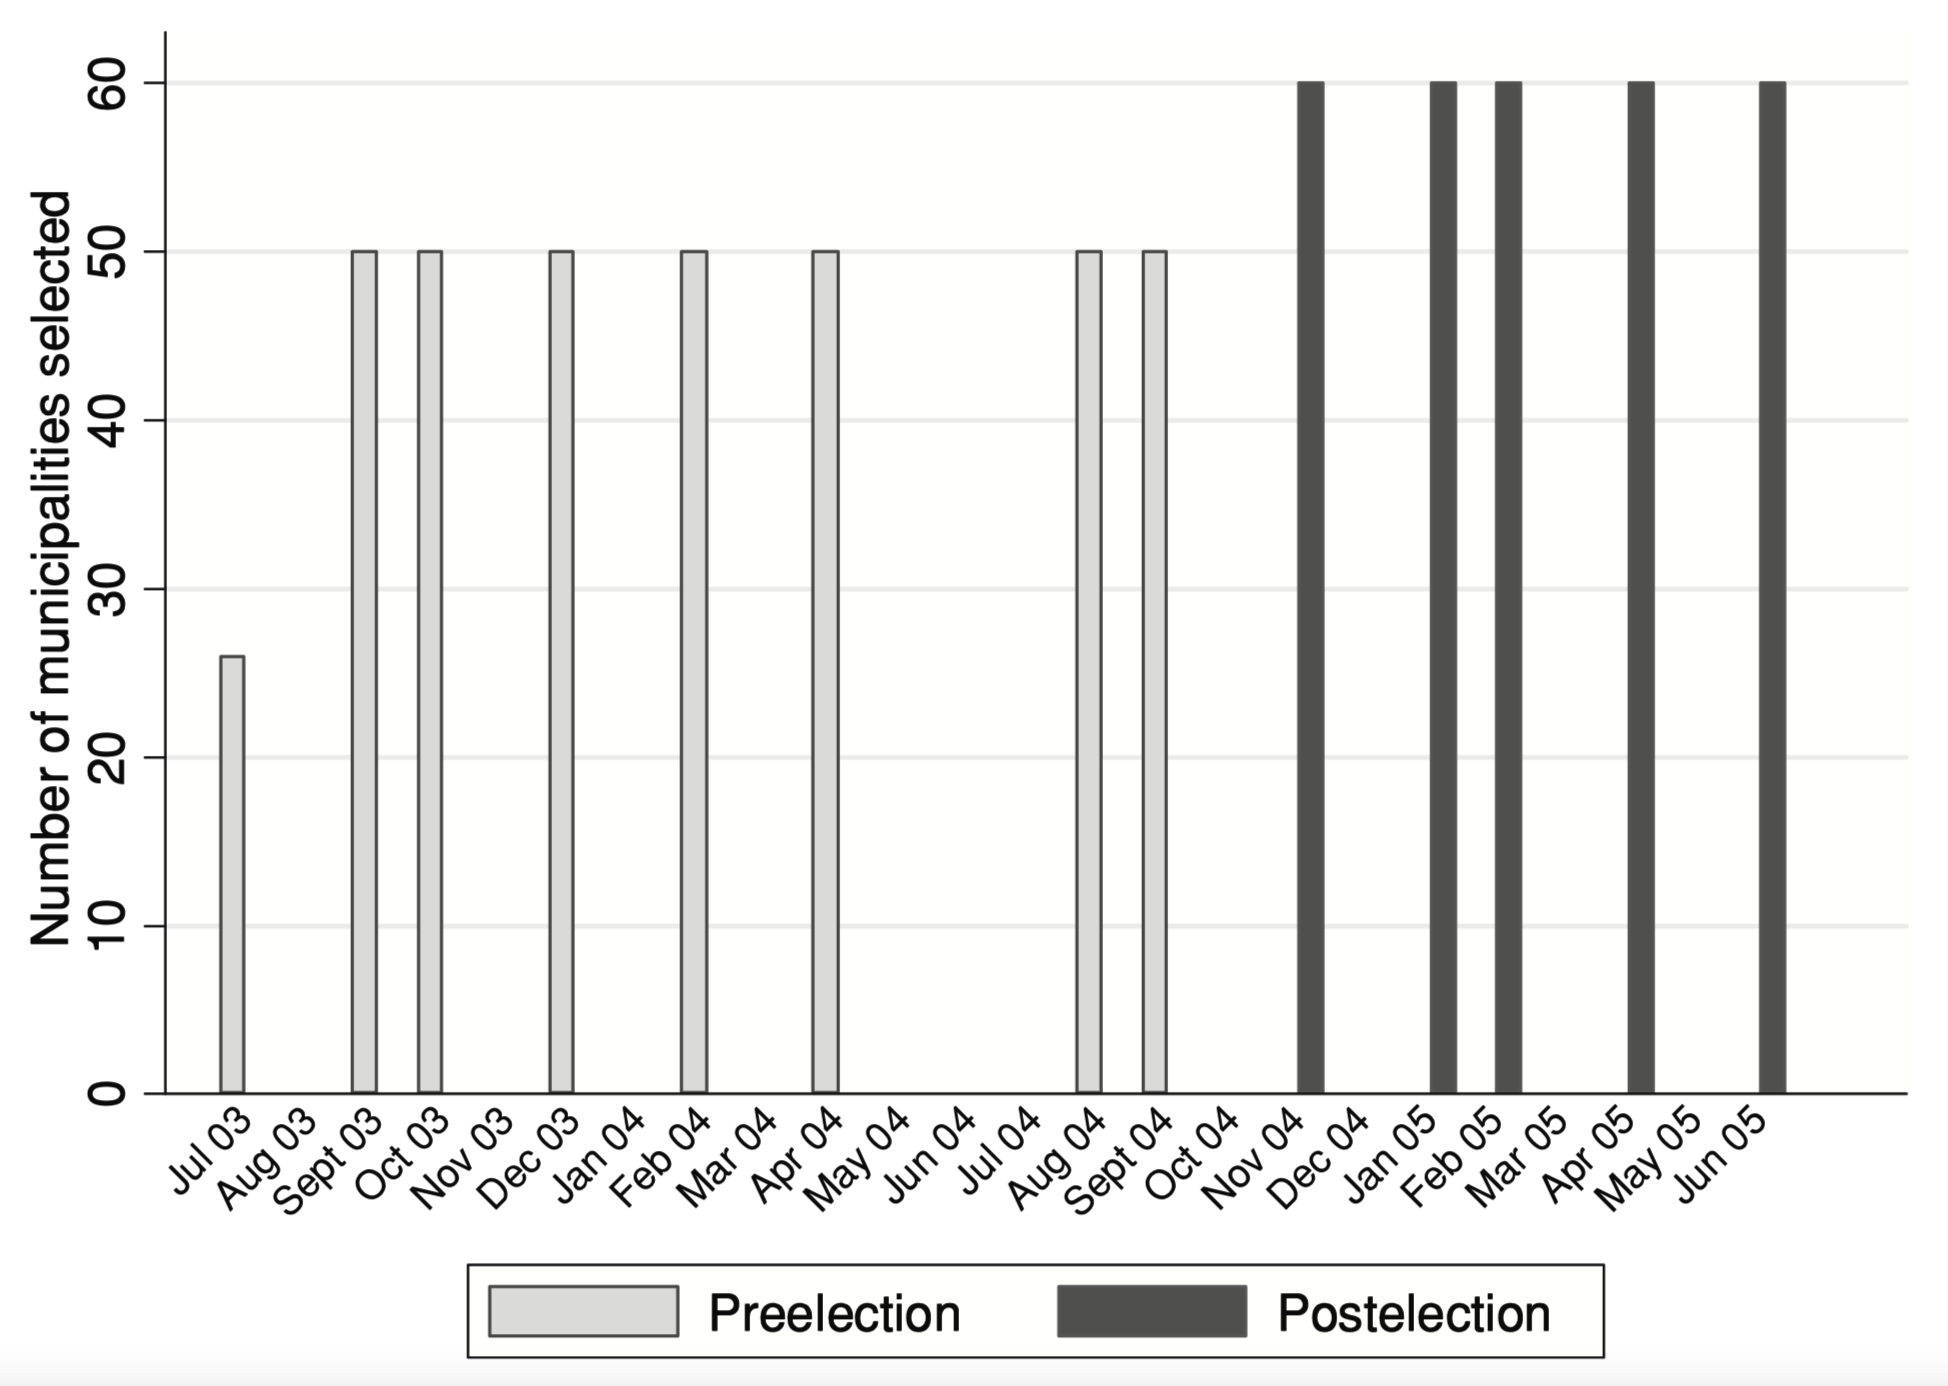
\includegraphics[height = 0.65 \textheight]{images/fig1.png}
        \caption{Program Timeline}
        \end{figure}
    \end{column}
    
    \begin{column}{0.4\textwidth}
    
    \begin{itemize}
      	\item<2-> sample: population \textbf<3->{\textcolor<3->{orange}{$<$450,000}}
      	\item<5-> selection by lottery
      	\item<6-> auditing process
      	\item<8-> audit report release
      \end{itemize}
    
    \only<3-4>{
    \begin{block}{\small \textbf{Important details}}
    \footnotesize
       \only<3-4>{\begin{itemize}
           \item<3-4> 92\% of all municipalities
           \item<3-4> 73\% of total population
           \item<4> excluding most state capitals/coastal cities
       \end{itemize}}
    \end{block}
    }
    
    \only<5>{
    \begin{block}{\small \textbf{Important details}}
    \footnotesize
       26 + 7$\times$50 + 5$\times$60 = 676 selections were made
       
       7 duplicated selections
       
       \textbf{669} municipalities were randomly selected 
    \end{block}
    }
    
    \only<6-7>{
    \begin{block}{\small \textbf{Important details}}
    \footnotesize
       \only<6-7>{\begin{itemize}
           \item<6-7> 10-15 auditors
           \item<6-7> 10 days of auditing
           \item<7> \textbf{validity}: hired competitively; well trained and paid; supervised
       \end{itemize}}
    \end{block}
    }
    
    \only<8-9>{
    \begin{block}{\small \textbf{Important details}}
    \footnotesize
       \only<8-9>{\begin{itemize}
           \item<8-9> reports: legislators/prosecutors
           \item<8-9> \textbf{summary}: \textbf<9>{\textcolor<9>{orange}{media}} and the Internet
           \item<9> {What form of media?} \textbf{\textcolor{orange}{radio}}
       \end{itemize}}
    \end{block}
    }
    
    \only<10-11>{\vspace{15pt}\textbf{\textcolor{orange}{Is the information really used by voters?}}}
    
    \only<11>{Yes, allegedly.}
    \end{column}
    \end{columns}
    \end{frame}
    
    \begin{frame}{\textit{Information:} The Measure of Corruption}
    
    \only<1-7>{
    \underline{What information is revealed on the audit reports}?
    \begin{itemize}
        \item<2-> \textbf{\textcolor{orange}{Quantitative:}} total amount of federal funds  transferred and the amount audited
        \item<3->\textbf{\textcolor{orange}{Qualitative:}} an itemized list describing each irregularity
    \end{itemize}}
    
    \begin{columns}[T]

    \begin{column}{0.3\textwidth}
        \uncover<4->{\begin{block}{\small \centering \textbf{Irregular procurement}}
        \uncover<5->{\footnotesize
        \begin{itemize}
            \item[-] no call for bids or minimum number of bids not attained
            \item[-] evidence of fraud
        \end{itemize}
        }
        \end{block}}
    \end{column}
    
    \begin{column}{0.3\textwidth}
        \uncover<4->{\begin{block}{\small \centering \textbf{Diversion of public funds}}
        \uncover<6->{\footnotesize
        \begin{itemize}
            \item[-] expenditure without proof
            \item[-] direct evidence of diversion
        \end{itemize}
        }
        \end{block}}
    \end{column}
    
    \begin{column}{0.3\textwidth}
        \uncover<4->{\begin{block}{\small \centering \textbf{Over-invoicing}}
        \uncover<7->{\footnotesize
        \begin{itemize}
            \item[-] purchase of public goods and services above the market price
        \end{itemize}
        }
        \end{block}}
    \end{column}
    
    \end{columns}
    
    \only<8->{
    \vspace{15pt}
    \underline{Construct a single measure}: the \textbf<9>{\textcolor<9>{orange}{total number of times}} each one of the three irregularities appears
    \begin{itemize}
        \small
        \item<10-> \textbf{\color{orange}Justification 1}: most common
        \item<11-> \textbf{\color{orange}Justification 2}: often complementary
        \item<12> {\footnotesize My interpretation: Layer 1 measure of corruption magnitude, could be more detailed, quantitatively}
    \end{itemize}
    }
        
    \end{frame}
    
    \begin{frame}{\textit{Political Consequence:} Municipal Election Results}
    \only<1->{
    \underline{Outcome: \textbf<2->{\textcolor<2->{orange}{Reelection results}}} 
    
    \begin{itemize}
        
        \item<3-> \textbf{\textcolor{orange}{Data source:}} Tribunal Superior Eleitoral (TSE)
        
        \item<3-> \textbf{\textcolor{orange}{Time frame:}} 2000 and 2004 voting results
        
        \item<3->
        \textbf{\textcolor{orange}{Voting information:}} Vote totals for each candidate by municipality
        
        \item<4-> \textbf{\textcolor{orange}{Sample selection:}} only first-term mayors eligible for reelection included
        
        \hspace*{\fill}\textbf<5->{(\textcolor<5->{orange}{373 municipalities}\only<5->{, 60\% of all mayors})}

    \end{itemize}}
        
    \end{frame}
    
    \begin{frame}{\textit{Covariates:} Candidate and Municipal Characteristics}
    \begin{itemize}
        \item<+-> Candidate characteristics from TSE
        \item<+-> Municipal characteristics from Brazilian Institute of Geography and Statistics (IBGE) 
        \begin{itemize}
            \item<+-> \textbf<6>{\textcolor<6>{orange}{2000}} population census: demographics
            \item<+-> \textbf<6>{\textcolor<6>{orange}{1999}} municipality survey: various controls
            \begin{itemize}
                \item public administration information: budgetary and planning procedures, public infrastructures, judiciary features, etc.
                \item measures of the \textbf<5->{\textcolor<5->{orange}{availability of media}}: the number of radio stations, daily newspapers, etc. 
            \end{itemize}
        \end{itemize}
        
    \end{itemize}
    
        
    \end{frame}